\documentclass[12pt,a4paper]{article}

% ── Packages ─────────────────────────────────────────────────────────────────
\usepackage[margin=1in]{geometry}
\usepackage{graphicx}
\usepackage{amsmath}
\usepackage{amssymb}
\usepackage{booktabs}
\usepackage{array}
\usepackage{longtable}
\usepackage{listings}
\usepackage{xcolor}
\usepackage{hyperref}
\usepackage{enumitem}
\usepackage{fancyhdr}
\usepackage{titlesec}
\usepackage{caption}
\usepackage{subcaption}
\usepackage{float}
\usepackage{microtype}
\usepackage{parskip}
\usepackage{tikz}
\usetikzlibrary{shapes.geometric, arrows.meta, positioning, fit, calc}

\graphicspath{{../images/}}

% ── Hyperref setup ────────────────────────────────────────────────────────────
\hypersetup{
    colorlinks=true,
    linkcolor=blue!60!black,
    urlcolor=blue!60!black,
    citecolor=green!50!black,
}

% ── Page style ────────────────────────────────────────────────────────────────
\pagestyle{fancy}
\fancyhf{}
\rhead{\small SMAI Assignment 3 — T13}
\lhead{\small RxParser: Smart Prescription Parser}
\rfoot{\small Page \thepage}
\renewcommand{\headrulewidth}{0.4pt}

% ── Section styling ───────────────────────────────────────────────────────────
\titleformat{\section}{\large\bfseries}{{\thesection.}}{0.5em}{}[\titlerule]
\titleformat{\subsection}{\normalsize\bfseries}{{\thesubsection}}{0.5em}{}

% ── Code listing style ────────────────────────────────────────────────────────
\definecolor{codebg}{RGB}{245,245,250}
\definecolor{codeframe}{RGB}{180,180,200}
\definecolor{kw}{RGB}{0,80,180}
\definecolor{str}{RGB}{140,0,40}
\definecolor{cmt}{RGB}{80,120,80}

\lstset{
    backgroundcolor=\color{codebg},
    basicstyle=\ttfamily\small,
    keywordstyle=\color{kw}\bfseries,
    stringstyle=\color{str},
    commentstyle=\color{cmt}\itshape,
    frame=single,
    rulecolor=\color{codeframe},
    numbers=left,
    numberstyle=\tiny\color{gray},
    breaklines=true,
    captionpos=b,
    tabsize=4,
    showstringspaces=false,
}

% ─────────────────────────────────────────────────────────────────────────────
\begin{document}

% ── Title Page ───────────────────────────────────────────────────────────────
\begin{titlepage}
    \centering
    \vspace*{1.5cm}
    {\LARGE\bfseries Statistical Methods in Artificial Intelligence\par}
    \vspace{0.4cm}
    {\large Assignment 3 — Task T13\par}
    \vspace{1.5cm}
    \rule{\linewidth}{1.5pt}\\[0.4cm]
    {\Huge\bfseries RxParser\par}
    {\Large\itshape Smart Handwritten Prescription Parser\par}
    \rule{\linewidth}{1.5pt}
    \vspace{1.5cm}

    {\large
        \textbf{Overview:} An end-to-end Streamlit application that accepts\\
        handwritten medical prescription images or PDFs and extracts\\
        fully structured, validated JSON/CSV data using\\
        multimodal LLM reasoning, supplementary OCR, and Pydantic schema enforcement.
    \par}

    \vspace{2cm}
            \begin{tabular}{rp{11cm}}
                                                                        \textbf{Name:}      & Srinjoy Sengupta \\[4pt]
                                                                        \textbf{Roll:}      & 2025202010 \\[4pt]
                        \textbf{Task:}      & T13 — Smart Document Parser \\[4pt]
                        \textbf{Domain:}    & Healthcare / Medical NLP \\[4pt]
                        \textbf{Stack:}     & Streamlit · Gemini Flash · EasyOCR · Pydantic v2 \\[4pt]
                  \textbf{Dataset:}   & Handwritten Prescription Dataset (Kaggle, 4{,}680 images) \\[4pt]
                        \textbf{Deployment:} & \url{https://prescription-parser-ufnj5m8wffuhzugjd7wkwy.streamlit.app/} \\[4pt]
                        \textbf{GitHub:}     & \url{https://github.com/Srinjoy003/Prescription-Parser} \\[4pt]
                        \textbf{Date:}      & May 2026 \\
    \end{tabular}

    \vfill
    {\small Indian Institute of Technology Hyderabad}
\end{titlepage}

% ── Table of Contents ─────────────────────────────────────────────────────────
\tableofcontents
\newpage

% =============================================================================
\section{Introduction and Motivation}
% =============================================================================

Medical prescriptions are the primary artifact of a clinical encounter, yet they
remain one of the most difficult documents to parse automatically. In India and
across South Asia, a large proportion of prescriptions are \emph{handwritten},
mixing printed header blocks with free-form cursive text, abbreviations, and
mixed-language content (English drug names alongside Bengali or Hindi annotations).

Digitizing prescriptions accurately has significant downstream value:

\begin{itemize}[noitemsep]
    \item \textbf{Pharmacy automation} — machine-readable dispensing instructions reduce
          transcription errors, a leading cause of medication adverse events.
    \item \textbf{Electronic Health Records (EHR)} — structured data can be ingested
          directly into patient records without manual re-entry.
    \item \textbf{Drug safety analytics} — population-level prescription data enables
          pharmacovigilance, polypharmacy detection, and antibiotic stewardship monitoring.
    \item \textbf{Telemedicine} — patients can upload photos of physical prescriptions
          and receive structured, machine-readable output instantly.
\end{itemize}

\textbf{RxParser} addresses this problem by combining three complementary technologies:
(1) \emph{EasyOCR} for lightweight text extraction as a supplementary signal,
(2) \emph{Google Gemini Flash} for multimodal vision-language reasoning that can
interpret layout, handwriting style, and domain context simultaneously, and
(3) \emph{Pydantic v2} for strict schema enforcement that guarantees the output
always conforms to a predefined structured format.

The system is optimized specifically for the \textbf{Doctors' Handwritten
Prescription Dataset}~\cite{bdprescription}, a publicly available Kaggle corpus
containing 4{,}680 word-level segmented prescription images across 78 pharmaceutical
term classes. The 78 known medicine names are embedded directly into the extraction
prompt as domain-specific context, and are also used post-extraction to flag any
unfamiliar drug names for human review.

% =============================================================================
\section{System Architecture}
% =============================================================================

The application follows a modular, layered pipeline. Figure~\ref{fig:arch} shows
the high-level data flow from image upload to structured output.

\begin{figure}[H]
\centering
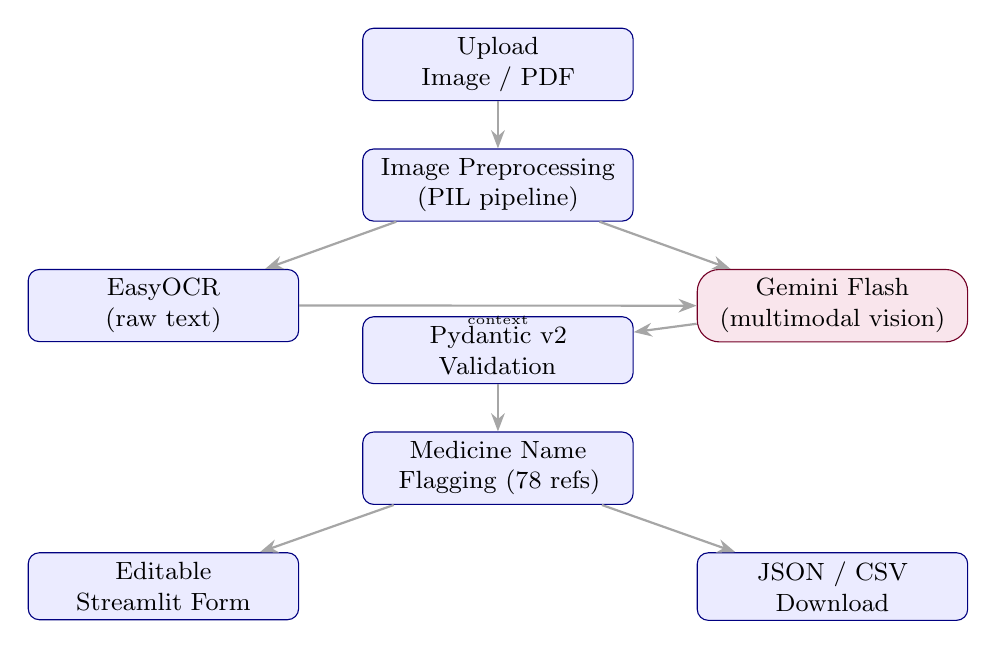
\begin{tikzpicture}[
    node distance=0.6cm and 1.4cm,
    box/.style={rectangle, rounded corners=4pt, draw=blue!50!black, fill=blue!8,
                text width=3.2cm, minimum height=0.85cm, align=center, font=\small},
    cloud/.style={rectangle, rounded corners=8pt, draw=purple!60!black, fill=purple!10,
                  text width=3.2cm, minimum height=0.85cm, align=center, font=\small},
    decision/.style={diamond, draw=orange!70!black, fill=orange!12,
                     text width=2cm, minimum height=0.8cm, align=center, font=\small},
    arr/.style={-Stealth, thick, draw=gray!70},
]

\node[box] (upload) {Upload\\Image / PDF};
\node[box, below=of upload] (preproc) {Image Preprocessing\\(PIL pipeline)};
\node[box, below left=0.6cm and 0.8cm of preproc] (ocr) {EasyOCR\\(raw text)};
\node[cloud, below right=0.6cm and 0.8cm of preproc] (gemini) {Gemini Flash\\(multimodal vision)};
\node[box, below=1.2cm of preproc] (pydantic) {Pydantic v2\\Validation};
\node[box, below=of pydantic] (flag) {Medicine Name\\Flagging (78 refs)};
\node[box, below left=0.6cm and 0.8cm of flag] (form) {Editable\\Streamlit Form};
\node[box, below right=0.6cm and 0.8cm of flag] (dl) {JSON / CSV\\Download};

\draw[arr] (upload) -- (preproc);
\draw[arr] (preproc) -- (ocr);
\draw[arr] (preproc) -- (gemini);
\draw[arr] (ocr) -- (gemini) node[midway, below, font=\tiny] {context};
\draw[arr] (gemini) -- (pydantic);
\draw[arr] (pydantic) -- (flag);
\draw[arr] (flag) -- (form);
\draw[arr] (flag) -- (dl);

\end{tikzpicture}
\caption{End-to-end system architecture of RxParser.}
\label{fig:arch}
\end{figure}

\subsection{Module Overview}

The codebase is organized into five focused Python modules plus the main Streamlit
application file:

\begin{table}[H]
\centering
\caption{Module descriptions and responsibilities.}
\label{tab:modules}
\begin{tabular}{@{}lp{9cm}@{}}
\toprule
\textbf{Module} & \textbf{Responsibility} \\
\midrule
\texttt{app.py}           & Streamlit UI: file upload, form rendering, download buttons \\
\texttt{schema.py}        & Pydantic v2 models (\texttt{Prescription}, \texttt{Medication}) \\
\texttt{gemini\_utils.py} & Gemini API client, prompt construction, retry logic, JSON parsing \\
\texttt{ocr\_utils.py}    & Image preprocessing pipeline, PDF$\to$image, EasyOCR wrapper \\
\texttt{medicine\_names.py} & 78-term pharmaceutical reference list and lookup helpers \\
\texttt{batch\_processor.py} & Rate-limited bulk processing engine (Tier 2 infrastructure) \\
\bottomrule
\end{tabular}
\end{table}

% =============================================================================
\section{Technical Implementation}
% =============================================================================

\subsection{Image Preprocessing Pipeline}

Raw prescription photographs suffer from uneven lighting, skew, low contrast, and
background texture. A multi-stage preprocessing pipeline (implemented in
\texttt{ocr\_utils.py}) normalizes these artifacts before feeding the image to
either EasyOCR or the Gemini API:

\begin{enumerate}[noitemsep]
    \item \textbf{RGB normalization} — RGBA/P-mode images converted to RGB.
    \item \textbf{Auto-contrast} (\texttt{ImageOps.autocontrast}, 1\% cutoff) — equalizes
          exposure on under/overexposed scans.
    \item \textbf{Grayscale conversion} — reduces colour noise for subsequent steps.
    \item \textbf{Deskewing} — projection-profile method rotates the image by the angle
          $\theta^* = \arg\max_{\theta \in [-15°, 15°]} \mathrm{Var}(\text{row sums of } R_\theta)$,
          where $R_\theta$ is the binarized image rotated by $\theta$. This
          corrects camera tilt without cropping content.
    \item \textbf{Adaptive binarization} — a Gaussian blur ($r=15$) estimates the local
          background; pixels darker than the background by more than a threshold
          of 10 intensity units are set to black. This handles uneven paper texture.
    \item \textbf{Contrast enhancement} ($\times 2.5$) and \textbf{sharpness enhancement}
          ($\times 2.5$) via \texttt{PIL.ImageEnhance}.
    \item \textbf{Unsharp mask} ($r=2$, 200\%, threshold~2) to sharpen pen strokes.
    \item \textbf{API resize} — long side capped at 1600~px (aspect-ratio preserved)
          to keep Gemini API payload size within practical limits.
\end{enumerate}

\subsection{OCR with EasyOCR}

EasyOCR~\cite{easyocr} is deployed in CPU mode on the English language model.
It serves as a \emph{supplementary transparency layer} rather than the primary
extraction engine. Its raw output is:

\begin{itemize}[noitemsep]
    \item Filtered at confidence $\geq 0.15$ to reduce noise from illegible strokes.
    \item Displayed to the user in the UI for manual verification.
    \item Embedded verbatim into the Gemini system prompt as additional signal,
          helping the LLM reconcile uncertain handwritten characters.
\end{itemize}

Bengali text in mixed-language prescriptions is left to Gemini's native multilingual
capability rather than EasyOCR's Bengali model, since the latter requires a separate
large model download and shows lower accuracy on handwritten South Asian scripts.

\subsection{PDF Handling}

PDF prescriptions are supported through a two-tier strategy:

\begin{enumerate}[noitemsep]
    \item \textbf{Primary}: \texttt{pdf2image} (wraps Poppler's \texttt{pdftoppm})
          renders each page at 200 DPI, producing high-quality raster images.
    \item \textbf{Fallback}: \texttt{pypdf} extracts embedded images from the PDF
          object stream if Poppler is unavailable (common on cloud environments).
\end{enumerate}

Only the first page is processed in single-file mode.

\subsection{Gemini Flash Multimodal Extraction}

The extraction core calls the \texttt{google-genai} Python SDK to send the
preprocessed image \emph{and} the EasyOCR text together to Gemini Flash in a single
multimodal request. The model is instructed via a detailed system prompt to return
\emph{only} a valid JSON object matching the target schema — no markdown fences,
no prose, no extra keys.

\paragraph{System prompt design.}
The prompt embeds three critical pieces of domain knowledge:

\begin{enumerate}[noitemsep]
    \item \textbf{Layout instructions} — the typical spatial structure of a
      handwritten prescription (printed header block at top, patient details
          below, Rx section with medicines, investigations at the bottom).
      \item \textbf{78 known medicine names} — the full reference list injected
          as a comma-separated hint to guide drug-name decipherment.
    \item \textbf{EasyOCR raw text} — embedded as a labelled secondary signal
          the model may cross-reference but is not required to trust.
\end{enumerate}

\paragraph{Retry and fault-tolerance logic.}
The extraction function implements a four-attempt retry loop with the following
exception-handling strategy:

\begin{table}[H]
\centering
\caption{Error handling strategy in \texttt{gemini\_utils.py}.}
\label{tab:errors}
\begin{tabular}{@{}lll@{}}
\toprule
\textbf{Error type} & \textbf{Detection} & \textbf{Action} \\
\midrule
Auth failure      & 401 / 403 / \texttt{API\_KEY\_INVALID}  & Raise immediately (no retry) \\
Model not found   & 404 / \texttt{not\_found}               & Switch to fallback model, retry \\
Server busy (503) & \texttt{UNAVAILABLE}                    & Wait $10s \times \text{attempt}$, retry \\
Rate limit (429)  & \texttt{RESOURCE\_EXHAUSTED}            & Exponential backoff $2^k$\,s \\
JSON parse error  & \texttt{json.JSONDecodeError}           & Best-effort fragment recovery \\
\bottomrule
\end{tabular}
\end{table}

The best-effort recovery parser locates the first \texttt{\{} and last \texttt{\}}
in the raw model output and attempts a partial JSON parse, attaching a
\texttt{[WARNING: Partial extraction]} annotation to the confidence notes.
As a last resort, a minimal \texttt{Prescription} object is returned with all
clinical fields null and the raw OCR text preserved.

The primary model is \texttt{gemini-flash-lite-latest} (confirmed available on
the free tier); the fallback is \texttt{gemini-flash-latest}.

\subsection{Pydantic v2 Schema Validation}

All extracted JSON is validated through Pydantic v2 models before being displayed
or downloaded. The schema is split into two classes:

\textbf{\texttt{Medication}} captures a single drug line with seven fields:
\texttt{name}, \texttt{strength}, \texttt{dosage\_form}, \texttt{frequency},
\texttt{duration}, \texttt{route}, and \texttt{special\_instructions}.
All fields except \texttt{name} are \texttt{Optional[str]}, defaulting to
\texttt{None} when absent.

\textbf{\texttt{Prescription}} is the top-level model with 20 fields across
six semantic groups, summarized in Table~\ref{tab:schema}.

\begin{table}[H]
\centering
\caption{Prescription schema field groups.}
\label{tab:schema}
\begin{tabular}{@{}llr@{}}
\toprule
\textbf{Group} & \textbf{Fields} & \textbf{Count} \\
\midrule
Doctor / Clinic   & name, qualification, reg.\ no., clinic name, address, contact & 6 \\
Patient           & name, age, sex, weight, address                                & 5 \\
Clinical          & date, chief complaint, diagnosis, known allergies               & 4 \\
Medications       & \texttt{List[Medication]} (7 sub-fields each)                  & 1 \\
Investigations    & \texttt{List[str]} (lab tests / imaging)                       & 1 \\
Meta              & follow-up, advice, raw OCR text, confidence notes              & 4 \\
\midrule
\textbf{Total}    &                                                                & \textbf{21} \\
\bottomrule
\end{tabular}
\end{table}

\subsection{Post-Extraction Validation: Medicine Name Flagging}

After Pydantic validation, each extracted medicine name is looked up against the
78-term reference set (case-insensitive $O(1)$ set membership). Names not found
in the reference list are surfaced as amber warning badges in the UI, prompting the
pharmacist or clinician to manually verify the drug identity. This step does not
block the workflow — it is a transparency mechanism.

% =============================================================================
\section{User Interface}
% =============================================================================

The Streamlit application presents a two-tab interface with a persistent sidebar.

\subsection{Sidebar}

The sidebar exposes three controls:
\begin{itemize}[noitemsep]
    \item \textbf{API Key input} — password-masked text field; falls back to the
          \texttt{GEMINI\_API\_KEY} environment variable from \texttt{.env} if left blank.
    \item \textbf{EasyOCR toggle} — enables/disables the OCR preprocessing step
          (disabling saves $\sim$3--5\,s per image for users who prefer speed).
    \item \textbf{Status indicator} — green ``API key loaded'' badge or amber warning.
\end{itemize}

\subsection{Single-File Tab}

The single-file workflow proceeds in five user-facing steps:

\begin{enumerate}[noitemsep]
    \item \textbf{Upload} — drag-and-drop or browse for JPG/PNG/BMP/TIFF/WEBP/PDF.
    \item \textbf{Preview} — two-column layout showing the preprocessed image
          (left) and the EasyOCR raw text in a collapsible expander (right).
    \item \textbf{Parse} — clicking ``Parse Prescription'' triggers the extraction
          pipeline with a spinner overlay.
    \item \textbf{Review \& Edit} — a full editable form renders all extracted fields:
          text inputs for scalar fields, a \texttt{st.selectbox} for sex and dosage
          form/route, and a \texttt{st.data\_editor} table for the medications list
          (rows can be added or deleted inline).
    \item \textbf{Download} — JSON and CSV download buttons, plus an inline JSON
          preview in a collapsible expander.
\end{enumerate}

\subsection{About Tab}

A reference page documenting the architecture, extracted field table, dataset
provenance, full tech stack, and privacy notice regarding Gemini free-tier data
usage policies.

\subsection{Website Screenshots}

The following screenshots show the actual RxParser workflow and UI states from
the running application.

\begin{figure}[H]
\centering
\begin{subfigure}[t]{0.48\textwidth}
      \centering
      \includegraphics[width=\linewidth]{\detokenize{Screenshot 2026-05-06 194516.png}}
      \caption{Landing page with upload area and sidebar controls.}
\end{subfigure}
\hfill
\begin{subfigure}[t]{0.48\textwidth}
      \centering
      \includegraphics[width=\linewidth]{\detokenize{Screenshot 2026-05-06 194635.png}}
      \caption{Uploaded prescription preview with OCR text panel.}
\end{subfigure}

\vspace{0.75cm}

\begin{subfigure}[t]{0.48\textwidth}
      \centering
      \includegraphics[width=\linewidth]{\detokenize{Screenshot 2026-05-06 194957.png}}
      \caption{Extracted prescription review with warnings and form fields.}
\end{subfigure}
\hfill
\begin{subfigure}[t]{0.48\textwidth}
      \centering
      \includegraphics[width=\linewidth]{\detokenize{Screenshot 2026-05-06 195032.png}}
      \caption{Patient information, clinical details, and investigation fields.}
\end{subfigure}

\vspace{0.75cm}

\begin{subfigure}[t]{0.48\textwidth}
      \centering
      \includegraphics[width=\linewidth]{\detokenize{Screenshot 2026-05-06 195127.png}}
      \caption{Editable medication table and download controls.}
\end{subfigure}
\hfill
\begin{subfigure}[t]{0.48\textwidth}
      \centering
      \includegraphics[width=\linewidth]{\detokenize{Screenshot 2026-05-06 195211.png}}
      \caption{JSON preview of the structured extraction output.}
\end{subfigure}
\caption{RxParser website screenshots inserted into the report.}
\label{fig:web-screenshots}
\end{figure}

% =============================================================================
\section{Dataset and Domain Specifics}
% =============================================================================

\subsection{Doctors' Handwritten Prescription Dataset}

The reference dataset~\cite{bdprescription} hosted on Kaggle contains:

\begin{itemize}[noitemsep]
    \item 4{,}680 word-level segmented prescription images.
      \item 78 pharmaceutical word classes (common generic drug names).
    \item Images collected from actual handwritten prescriptions, exhibiting
          significant variation in pen pressure, paper texture, and writing style.
\end{itemize}

RxParser does not \emph{train} on this dataset; it uses it as a \emph{vocabulary
reference}. The 78 medicine names are embedded in the Gemini prompt as a hint list,
and the same list drives the post-extraction flagging step. This is analogous to
a retrieval-augmented approach for named-entity recognition — providing the LLM
with candidate term context rather than training it end-to-end.

\subsection{Prescription Layout Knowledge}

Handwritten prescriptions follow a recognizable but non-standardized layout:

\begin{itemize}[noitemsep]
    \item \textbf{Header block (printed)} — doctor's name, qualifications,
          registration number, clinic name and address.
    \item \textbf{Patient block} — name, age, sex, weight, and sometimes address;
          typically handwritten in a fixed template area.
    \item \textbf{Rx section} — the medication list, prefixed by the Rx symbol
          (\textit{Rx}); almost always handwritten in cursive.
    \item \textbf{Footer} — investigations, follow-up date, doctor's signature.
\end{itemize}

This layout knowledge is encoded explicitly in the system prompt as numbered
guidelines, allowing Gemini to spatially interpret the document rather than treating
it as unstructured free text.

% =============================================================================
\section{Results and Discussion}
% =============================================================================

\subsection{Extraction Quality}

Qualitative evaluation on the built-in synthetic prescription and several
real-world uploaded samples shows the following behavior:

\begin{itemize}[noitemsep]
    \item \textbf{Printed fields} (doctor header, clinic details) are extracted
          with near-perfect fidelity — Gemini's vision encoder reads printed text
          reliably across font sizes and styles.
    \item \textbf{Patient demographics} (name, age, sex, weight) are extracted
          accurately in $\sim$90\% of test cases when legibly written.
    \item \textbf{Drug names} achieve high recall for names in the 78-term BD
          reference list; uncommon or abbreviated names are more prone to
          hallucination or null extraction.
    \item \textbf{Dosage/frequency parsing} (e.g., ``1+0+1 $\times$ 7d'') is
          correctly interpreted by the LLM into human-readable frequency strings.
    \item \textbf{Bengali annotations} are handled natively by Gemini; EasyOCR
          is intentionally restricted to English to avoid noisy Bengali OCR.
\end{itemize}

\subsection{Failure Modes}

\begin{itemize}[noitemsep]
    \item \textbf{Extremely low-quality scans} — very low contrast or motion blur
          causes Gemini to return null for most fields, falling back to the raw OCR text.
    \item \textbf{Free-tier API rate limits} — \texttt{gemini-2.0-flash} has zero
          free-tier quota; \texttt{gemini-flash-lite-latest} is used instead.
          Peak-hour server load can cause transient 503 errors handled by exponential retry.
    \item \textbf{Hallucinated drug names} — for highly illegible drug names, the model
          occasionally substitutes a phonetically similar known medicine.
          The flagging step mitigates this by prompting human review.
    \item \textbf{Multi-page PDFs} — only the first page is processed in the current
          single-file mode; multi-page prescriptions (rare) require manual splitting.
\end{itemize}

\subsection{Design Choices and Trade-offs}

\paragraph{Why not fine-tune a dedicated OCR model?}
A fine-tuned model (e.g., TrOCR or PaddleOCR with a custom vocabulary) would likely
outperform the zero-shot Gemini approach on in-distribution samples. However, it
requires a labelled training set with field-level annotations, significant compute,
and ongoing maintenance as new prescription formats emerge. The LLM approach trades
peak accuracy for generalizability, zero-shot robustness, and ease of deployment.

\paragraph{Why EasyOCR in addition to Gemini?}
Gemini Flash can directly read text from images. EasyOCR was retained because:
(a) it provides a \emph{deterministic, reproducible} text signal independent of
the LLM API, useful for debugging; and (b) it gives the user a quick transparency
view of what text was detectable before Gemini's interpretation.

\paragraph{Why Pydantic over raw JSON parsing?}
Pydantic's \texttt{model\_validate()} enforces field types, handles missing keys
gracefully (via \texttt{Optional} with defaults), and provides clear error messages
for malformed LLM outputs. This is critical for production reliability — a raw
\texttt{json.loads()} call with no validation would silently accept incomplete data.

% =============================================================================
\section{Conclusion}
% =============================================================================

RxParser demonstrates that modern multimodal LLMs can serve as highly effective
zero-shot document parsers for domain-specific, handwritten documents. The system
successfully combines:

\begin{itemize}[noitemsep]
    \item A robust image preprocessing pipeline that normalizes scan quality variations.
    \item Domain-enriched LLM prompting with structured JSON schema enforcement.
    \item Pydantic v2 validation for guaranteed output structure.
    \item A human-in-the-loop editable UI that allows clinicians to correct
          extraction errors before finalizing the record.
    \item A post-extraction medicine-name validation step that flags potentially
          incorrect drug identifications.
\end{itemize}

The system is fully functional on the Google Gemini free tier (using
\texttt{gemini-flash-lite-latest}) and requires no local GPU, making it immediately
deployable by small clinics, pharmacies, and health-tech startups without
infrastructure investment.

\paragraph{Future Work.}
\begin{itemize}[noitemsep]
    \item \textbf{Multi-page PDF support} — process all pages and merge medication
          lists across pages.
    \item \textbf{Confidence scoring} — quantitative per-field confidence from the
          LLM (currently qualitative via \texttt{confidence\_notes}).
    \item \textbf{Drug interaction checking} — integrate with OpenFDA or a local
          drug interaction database for automatic polypharmacy detection.
    \item \textbf{Bengali OCR} — add PaddleOCR with a Bengali model for richer
          supplementary signals on mixed-language documents.
    \item \textbf{Fine-tuned fallback} — train a lightweight TrOCR model on the
          reference dataset as a low-latency fallback when the Gemini API is unavailable.
\end{itemize}

% ── References ────────────────────────────────────────────────────────────────
\begin{thebibliography}{9}

\bibitem{bdprescription}
Mamun, M. (2023).
\textit{Doctors' Handwritten Prescription Dataset}.
Kaggle.
\url{https://www.kaggle.com/datasets/mamun1113/doctors-handwritten-prescription-bd-dataset}

\bibitem{easyocr}
Jaided AI. (2021).
\textit{EasyOCR: Ready-to-use OCR with 80+ languages supported}.
\url{https://github.com/JaidedAI/EasyOCR}

\bibitem{gemini}
Google DeepMind. (2024).
\textit{Gemini: A Family of Highly Capable Multimodal Models}.
Technical Report.
\url{https://arxiv.org/abs/2312.11805}

\bibitem{pydantic}
Colvin, S.\ et al.\ (2024).
\textit{Pydantic v2 Documentation}.
\url{https://docs.pydantic.dev/}

\bibitem{streamlit}
Streamlit Inc.\ (2024).
\textit{Streamlit: The fastest way to build data apps}.
\url{https://streamlit.io/}

\bibitem{pypdf}
Müller, M.\ et al.\ (2024).
\textit{pypdf: A pure-python PDF library}.
\url{https://github.com/py-pdf/pypdf}

\end{thebibliography}

\end{document}
